\documentclass[nofootinbib,twocolumn,showpacs,prl,superscriptaddress,secnumarabic,amssymb,nobibnotes,aps,floatfix]{revtex4}
\usepackage{graphicx}
\usepackage{hyperref}
\usepackage{amsmath}
\usepackage{dcolumn}% Align table columns on decimal point
\usepackage{bm}% bold math

%
\def\Dirac#1{#1\hskip-5pt/}
%
\begin{document}

\title{First Exclusive Measurement of Deep Virtual Compton Scattering off $^4$He: Toward the 3D tomography of nuclei}

\newcommand*{\ANL}{Argonne National Laboratory, Argonne, Illinois 60439}
\newcommand*{\ANLindex}{1}
\affiliation{\ANL}
\newcommand*{\ORSAY}{Institut de Physique Nucl\'eaire, CNRS/IN2P3 and Universit\'e Paris Sud, Orsay, France}
\newcommand*{\ORSAYindex}{2}
\affiliation{\ORSAY}
\newcommand*{\JLAB}{Thomas Jefferson National Accelerator Facility, Newport News, Virginia 23606}
\newcommand*{\JLABindex}{3}
\affiliation{\JLAB}
 
\newcommand*{\NOWJLAB}{Thomas Jefferson National Accelerator Facility, Newport News, Virginia 23606}
\newcommand*{\NOWODU}{Old Dominion University, Norfolk, Virginia 23529}
 %%%%%%%%%%%%%%% END OF Latex Macros for institute addresses  %%%%%%%%%%%%%%%%%%%%%%%%% 

\author {M.~Hattawy}
\affiliation{\ANL}
\affiliation{\ORSAY}
\author {R.~Dupr\'{e}} 
\affiliation{\ANL}
\affiliation{\ORSAY}
\author {N.A.~Baltzell} 
\affiliation{\ANL}
\affiliation{\JLAB}
\author {K.~Hafidi} 
\email[corresponding author: ]{kawtar@anl.gov}
\affiliation{\ANL}


\collaboration{The CLAS Collaboration}
\noaffiliation

%
\date{\today}
%
\begin{abstract}
We report the first fully exclusive measurement of deeply virtual Compton 
scattering (DVCS) off a nucleus for $A>1$. The experiment used the 6 GeV 
electron beam from Jefferson Lab projected onto a $^4$He target in the center of the CEBAF 
Large Acceptance Spectrometer (CLAS). An additional radial time projection 
chamber (RTPC) was used to detect the recoiling $^4$He nuclei and ensure the 
exclusivity of the process. We measured beam spin asymmetries significantly
larger than the one observed on proton targets and extract,
in a completely model independent way, the chiral even generalized parton 
distribution (GPD) of the $^4$He nucleus. This pioneering measurement 
leads the way toward the 3D imaging of the partonic structure of nuclei.
\end{abstract}
\pacs{Valid PACS appear here}

\maketitle 

A wealth of information on the quantum chromodynamics (QCD) lies in the 
internal structure of hadrons. In the recent past, the development of the 
generalized parton distributions (GPDs) framework has offered the possibility
to obtain new information about the momentum and spatial degrees of 
freedom of the quark and gluons inside hadrons [Add ref Mueller, Ji, Rad.]. 
In impact parameter space, the GPDs are indeed interpreted as a tomography of the 
transverse plane for partons carrying a certain longitudinal momentum 
\cite{Burkardt:2000za,Diehl:2002he,Belitsky:2002ep}. 

The main access to GPDs is through the measurement of deep virtual Compton 
scattering (DVCS), i.e. the hard exclusive electroproduction of a real photon. 
While other processes are known to be sensitive to GPDs, the measurement of the
DVCS is considered as the cleanest probe and has been the focus of a worldwide effort 
\cite{Stepanyan:2001sm,Airapetian,Chekanov:2003ya,Aktas:2005ty,Chen:2006na,Munoz 
Camacho:2006hx,Girod:2007aa,Gavalian:2009,Seder:2015,Pisano:2015,Jo:2015ema} 
[Should we cite less publications on the topic or a review?]
involving several accelerator facilities such as Jefferson Lab (JLab), HERA and  
CERN. The vast majority of these measurements was focused on the study of the 
proton structure and allow the extraction of the tomography of the nucleon [refs].

This framework is also applicable to nuclei, giving access to completely new 
information about the nuclear structure in terms of quarks and gluons[refs to add].
The study of the 3D structure of the nuclei appears to be especially important
in light of the large nuclear effects observed in nuclear parton distribution 
functions [ref to EMC reviews]. Experimentally, the coherent DVCS channel is 
difficult to measure because of its small cross section and the necessity to
ensure that the target remains intact while emitting a hard photon 
($eA \rightarrow e' A' \gamma$). Figure \ref{fig:diags} illustrates the 
hand bag diagram for the coherent DVCS on $^4$He.  

\begin{figure}[tb]
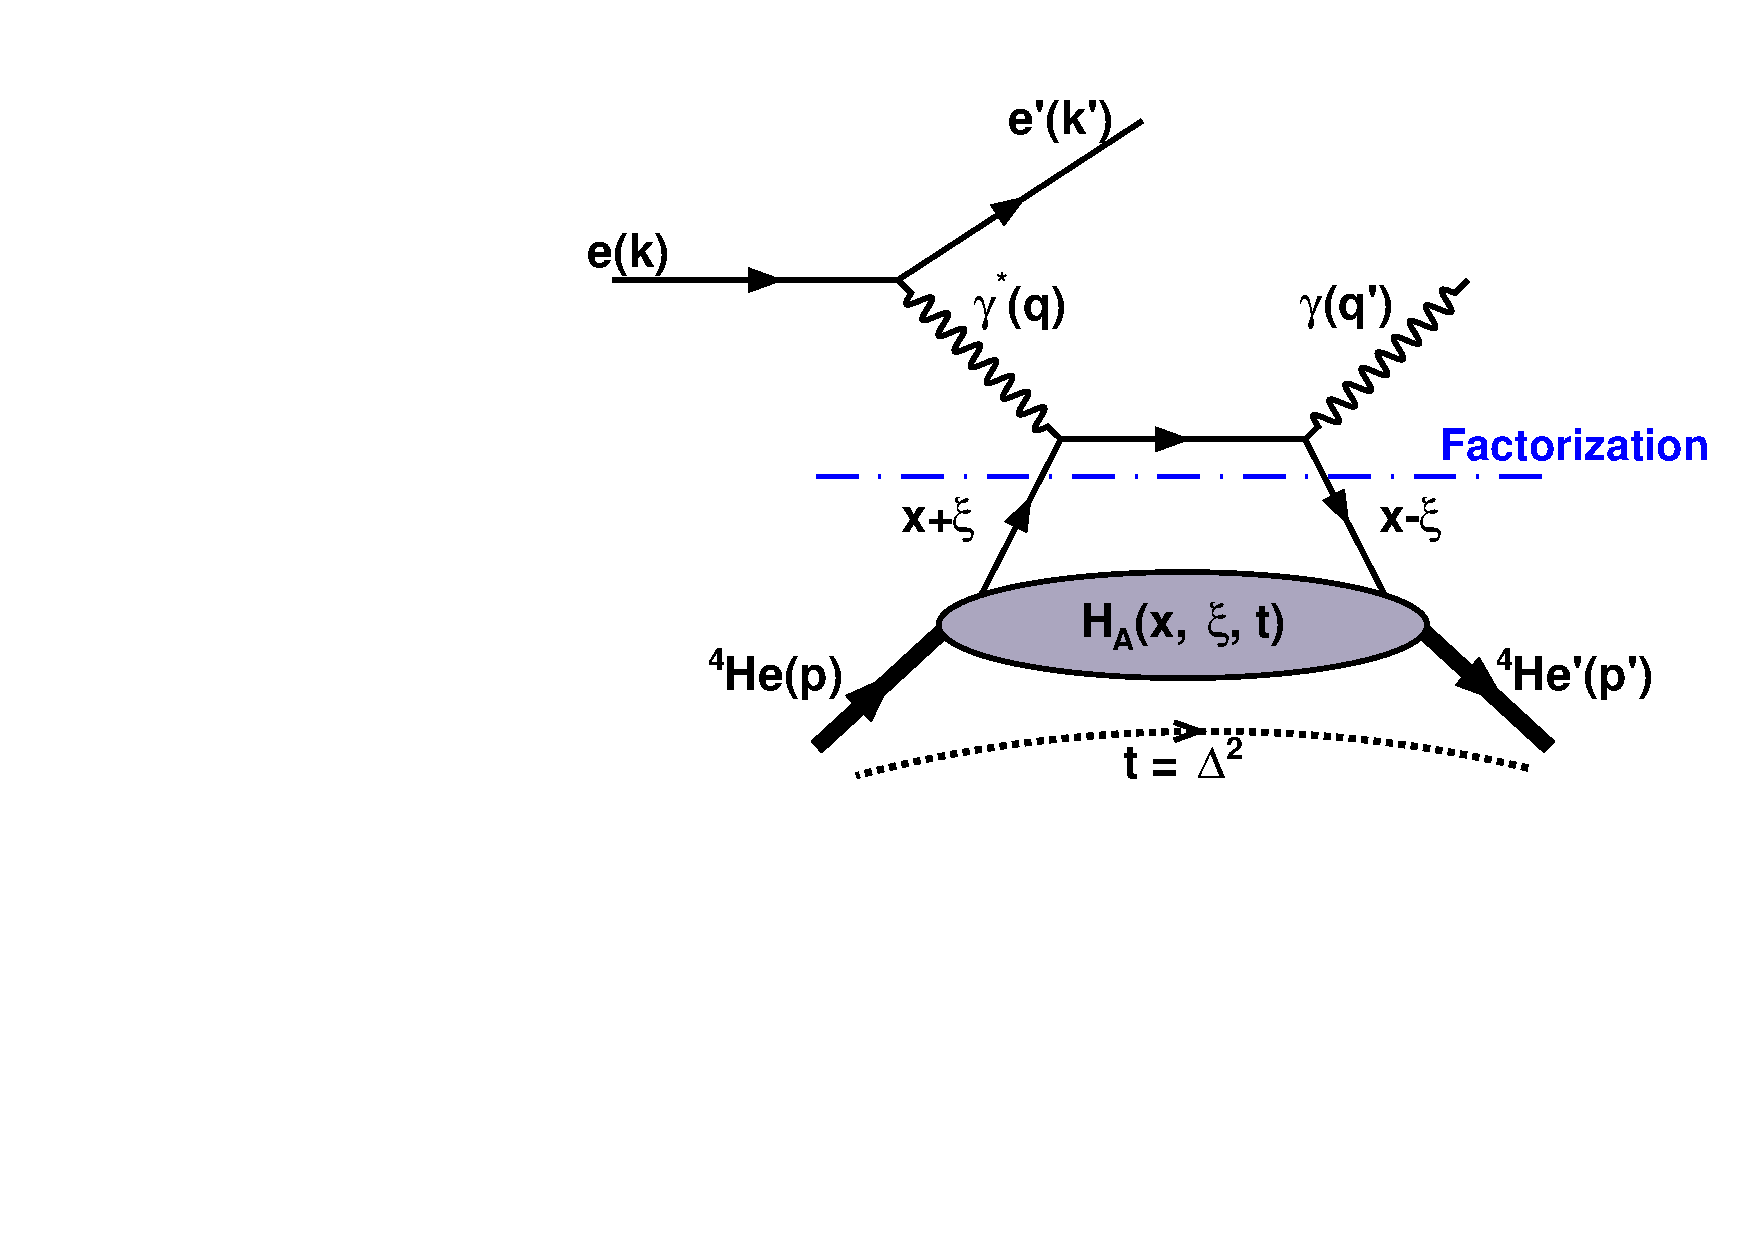
\includegraphics[width=6.5cm]{figs/DVCS_diagram.pdf}
\caption{Representation of the leading-order, twist-2, handbag diagram of the 
DVCS process off $^4$He.}
\label{fig:diags}
\end{figure}

Similarly to the proton case, at large photon's 4-momentum square  
$Q^2$ ($= -(k-k')^{2}$) and small squared momentum transfer $t$ ($= 
(p-p')^{2}$), the DVCS handbag diagram can be factorized into two parts 
\cite{Freund_Collins,Ji_Osborne}. The hard part includes photons-quark 
interaction and is calculable with perturbative QED, while the 
soft/non-perturbative part is parametrized in terms of GPDs, which embed the 
partonic structure of the hadron. 

The GPDs are defined for each quark flavor and gluon as matrix
elements of the light cone operators \cite{Belitsky}, describing the transition 
between the initial and final states of a hadron. The GPDs depend on two 
longitudinal momentum fraction variables ($x$, $\xi$) and on the momentum 
transfer $t$ to the target. $x$ is the average longitudinal momentum fraction 
of the parton involved in the process and $\xi$ is the longitudinal fraction of 
the momentum transfer $t$, which is related to the Bjorken variable $x_{B}$: 
$\xi\approx {{x_B}\over{2-x_B}}$, where $x_B=\frac{Q^2}{2M\nu}$ with
the proton mass $M$ and $\nu=E_e-E_{e^\prime}$. The GPDs $x$ variable cannot be 
measured experimentally in a DVCS reaction. Hence, we measure the their 
convolutions on $x$, the so-called Compton Form Factors (CFF) 
\cite{Guidal:2013rya}.  In a DVCS process, the number of GPDs needed to 
parametrize the partonic structure of a hadron depends on the different 
configurations between the spin of the hadron and the helicity direction of the 
struck quark.  Therefore, the partonic structure of spin zero nuclei, such as 
$^4He$ and $^{12}C$, is parametrized by only one GPD ($H_{A}(x,\xi,t)$) at 
leading twist, while 4 GPDs arise in the nucleon case.  In this work, we have 
chose the $^4$He nucleus as our target of interest because of it's spinless 
nature and it shows a clear EMC effect \cite{JSeely}, in addition of having a 
high density and it is a well-known few-body system.

The study of nuclear DVCS is still in its infancy due to the challenging 
detection of the low-energy recoil nuclei in fixed target experiments. Until 
very recently, the HERMES experiment \cite{Ellinghaus:2002zw} was the only one 
to measure DVCS off heavier nuclei such as $^4$He, N, Ne, Kr and Xe, where only 
the scattered electron and the real photon are detected. In this paper, we 
report the first exclusive measurements of the coherent DVCS channel off $^4$He 
where all products of the reaction are detected including the recoiling $^4$He 
nucleus. Following this exclusive measurement, the $^4$He CFF 
($\mathcal{H}_{A}$) will be extracted experimentally in a fully model 
independent way for the first time ever. The incoherent DVCS channel 
measurement from the same data set in in preparation and will reported in 
another publication. 

This work presents the first exclusive measurement of the beam-spin asymmetry 
of the reaction $e~^{4}He\rightarrow e'~^{4}He~\gamma$.This DVCS sensitive 
observable is measurable using a polarized lepton beam on an unpolarized target 
(U). It is convenient to use the beam-spin asymmetry as a DVCS observable 
because most of the experimental normalization and acceptance issues cancel out 
in the asymmetry ratio. It is defined in terms of the cross sections as:
  \begin{equation}
  A_{LU} = \frac{d^{5}\sigma^{+} - d^{5}\sigma^{-} }
                {d^{5}\sigma^{+} + d^{5}\sigma^{-}}.
    \label{BSA_equation}
  \end{equation}
where $d^{5}\sigma^{+}$($d^{5}\sigma^{-}$) is the DVCS differential cross 
section for a positive (negative) beam helicity. Experimentally, the DVCS 
reaction is indistinguishable from the Bethe-Heitler (BH) process, where the 
final photon is emitted either from the incoming or the outgoing leptons. The 
BH process is not sensitive to GPDs and does not carry information about the 
partonic structure of the hadronic target, and it's amplitude is calculable 
from the well-known electromagnetic form factors.

At leading twist order, the photon-electroproduction cross section can be 
decomposed into a BH, a DVCS, and an interference terms. The amplitudes of the 
three terms is approximated as a finite sum of Fourier harmonics, the so-called 
BMK approximation, as shown for the nucleon DVCS in \cite{Belitsky:2001ns} and 
for the spinless nuclei in \cite{Kirchner:2003wt,Belitsky:2008bz}. Therefore, 
the beam-spin asymmetry ($A_{LU}$) with the two opposite helicities of a 
longitudinally-polarized electron beam (L) on a spin-zero target (U) can be 
simplified as:
\small
\begin{equation}
\begin{split}
A_{LU}(\phi) =~~~~~~~~~~~~~~~~~~~~~~~~~~~~~~~~~~~~~~~~~~~~~~~~~~~~~~~~~\\
 \frac{\alpha_{0}(\phi) \, \Im m(\mathcal{H}_{A})}
{\alpha_{1}(\phi) + \alpha_{2}(\phi) \, \Re e(\mathcal{H}_{A}) + \alpha_{3}(\phi) \, 
\big( 
\Re e(\mathcal{H}_{A})^{2} + \Im m(\mathcal{H}_{A})^{2} \big)}
\label{eq:A_LU-coh}
\end{split}
\end{equation}
\normalsize
where $\Im m(\mathcal{H}_{A})$ and $\Re e(\mathcal{H}_{A})$ are the imaginary 
and real parts of the $^4$He CFF $\mathcal{H}_{A}$ associated to the GPD $H_A$. 
$\phi$ is the azimuthal angle between the ($e$,$e'$) and 
($\gamma^{*}$,$^4$He$'$) planes. The $\alpha_{i}$'s are $\phi$-dependent 
kinematical factors that depend on the nuclear form factor ($F_{A}(t)$) and the 
independent variables $Q^2$, $x_{B}$ and $t$. These factors are simplified as:
\small
\begin{eqnarray}
   \alpha_0 (\phi) & = &\frac{x_{A}(1+\epsilon^2)^2}{y} S_{++}(1) \sin(\phi)\\
    \alpha_1 (\phi) & = & c_0^{BH}+c_1^{BH} \cos({\phi})+c_2^{BH} \cos(2\phi)\\ 
   \alpha_2 (\phi) & = & \frac{x_{A}(1+\epsilon^2)^2}{y}  \left( C_{++}(0) +  
C_{++}(1) cos(\phi) \right)\\
\alpha_3 (\phi) &=& \frac{x^{2}_{A}t(1+\epsilon^2)^2}{y} {\mathcal P}_1(\phi) 
{\mathcal P}_2(\phi) \cdot 2 \frac{2-2y+y^2 + \frac{\epsilon^2}{2}y^2}{1 + 
\epsilon^2}
\end{eqnarray}
\normalsize

Where $x_{A} = \frac{x_{B}M_{N}}{M_{A}}$ with $M_{A}$ is the $^4$He mass, 
$\mathcal{P}_1(\phi)$ and $\mathcal {P}_2(\phi)$ are the Bethe-Heitler
propagators. The factors: $c_{0,1,2}^{BH}$, $c_0^{DVCS}$, $c_{0,1}^{INT}$ and
$s_1^{INT}$ are the Fourier coefficients of the BH, $S{++}(1)$, $C_{++}(0)$, 
and $C_{++}(1)$ are the Fourier harmonics in the leptonic tensor. Their 
explicit expressions can be found in \cite{Belitsky:2008bz}.  Therefore, Using 
the $\alpha_{i}$ factors, one can obtain in a totally model-independent way 
$\Im m(\mathcal{H}_{A})$ and $\Re e(\mathcal{H}_{A})$ from fitting the 
experimental $A_{LU}$ as a function of $\phi$ for given values of $Q^2$, 
$x_{B}$, and $t$.

%experimental setup

The experiment, CLAS-EG6, took place in the experimental Hall-B of Jefferson 
laboratory (JLab) in 2009. JLab delivers, simultaneously, a nearly 100\% duty 
factor polarized electrons into three experimental Halls (A, B, C). The data 
were collected over three months via projecting a 6.064 GeV longitudinally 
polarized beam, (83$\%$ polarization), on a 6 atm gaseous $^4$He target.  The 
Hall-B Large Acceptance Spectrometer (CLAS) basic design \cite{CLAS_ref} was 
supplemented, during the CLAS-E1DVCS1 experimental run \cite{Girod:2007aa} in 
2005, with a specially designed electromagnetic calorimeter, Inner calorimeter 
(IC). The IC has extended the photon detection acceptance of CLAS, which is 
originally from 15$^{\circ}$ to 45$^{\circ}$, to polar angle reach as minimum 
as 4$^{\circ}$.  During the same experiment, a 5 Tesla solenoid was added 
around the target to shield the inner detectors from the low-energy M\o ller 
electrons.

At 6 GeV incident electron beam energy, the recoil $^4$He nuclei, from the 
coherent DVCS channel, have an average momentum (per charge) around 125 MeV/c, 
while the CLAS spectrometer detects charged particles with a threshold of 250 
MeV/c. In order to ensure the exclusivity of the our coherent DVCS channel, we 
built a small and light radial time projection chamber (RTPC) to detect 
recoiling nuclei down to energies of few MeVs. Figure~\ref{fig:RTPC} presents 
our cylindrical RTPC, which is 20 cm long and 15 cm diameter, surrounding the 
$^4$He gaseous target and being inside the available space inside the solenoid 
, with a 3 cm radial drift length. The detector was specifically calibrated for 
$^4$He nuclei using elastic scattering produced with a 1.2~GeV electron beam.


\begin{figure}[tb]
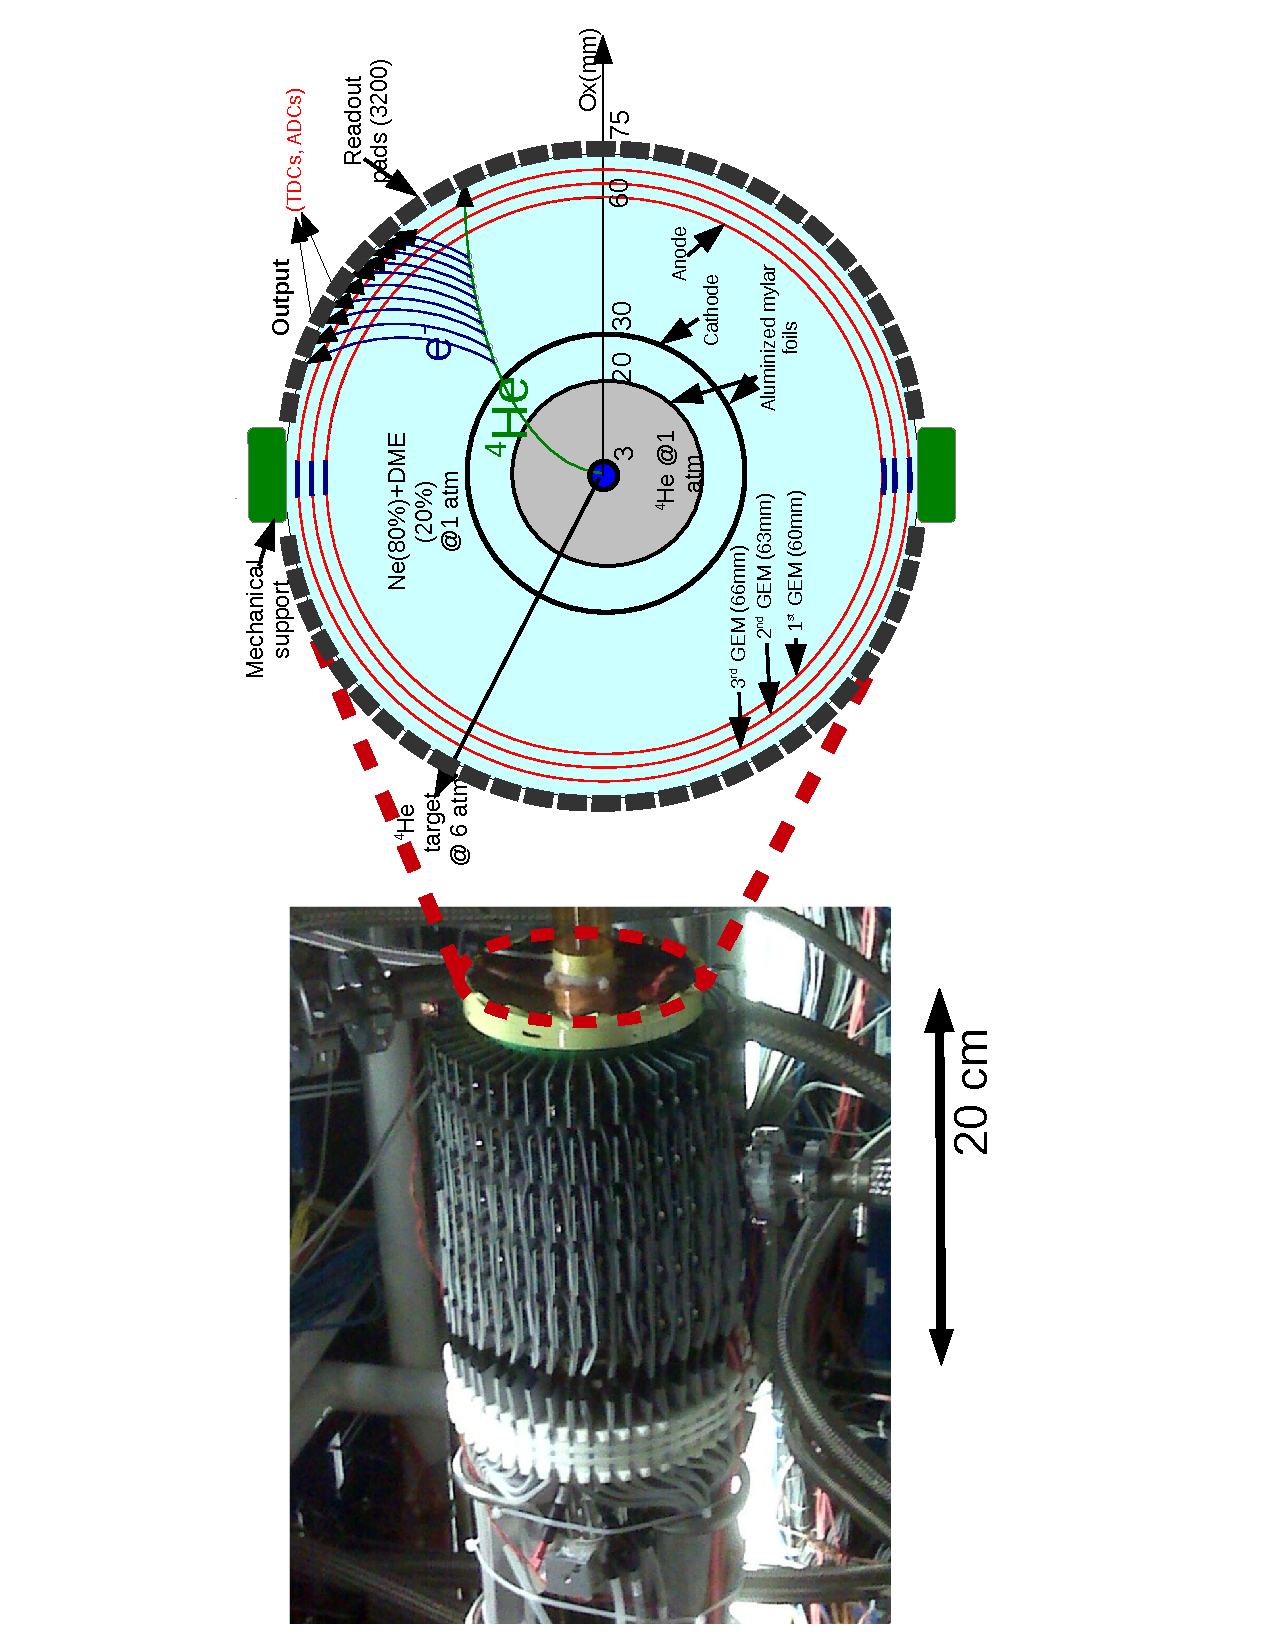
\includegraphics[width=7.0cm,angle=-90]{figs/RTPC.pdf}
\vspace{-1.1cm}
\caption{Left: A picture of the CLAS-EG6 RTPC before insertion into the 
   solenoid. Right: A cross section of the CLAS-EG6 RTPC perpendicular to the 
   beam direction. An illustration of a $^4$He track originating from the 
   pressurized straw target is shown along with the electrons produced in the 
drift region.}
\label{fig:RTPC}
\end{figure}

%DVCS selection
Identifying the coherent DVCS candidates is the first step of the data 
analysis. These events have one electron, one $^4$He, and at least one photon 
in the final state. Electrons were identified by passing the fiducial cuts and 
having signals in all the sub-detectors of CLAS spectrometer (drift chambers, 
Cherenkov counters, the standard CLAS electromagnetic calorimeter, and 
scintillators). $^4$He tracks were identified by passing all the geometrical, 
timing and quality cuts in the RTPC detector. In principle, with constant beam 
luminosity, target density and pressure, the event rate has to be constant over 
the experimental time. Due to the changes in the experimental conditions, such 
as changing a trigger in a detector, a slight shift in the beam position or a 
system failure somewhere, this rate changes. We minimize the effects of these 
changes on the reconstructed events by selecting the good runs. To this aim, we 
monitor the ratio between the number of the good tracks reconstructed in the 
RTPC to number of the detected good electrons in the CLAS detector as a 
function of run number \cite{eg6_note}.

Even though the DVCS reaction has only one real photon in the final state, 
events with more than one good photon are not discarded at this stage. This is 
motivated by the fact that some photons correspond to random coincidences and 
discarding these events results in losing good events. Then, events with one or 
more $\pi^{0}$ are removed from the coherent DVCS sample. After that, the most 
energetic IC photon was considered as the DVCS photon candidate. Next, a 
$Q^{2}>1~[GeV^{2}/c^{2}]$ cut is applied on the DVCS candidates in order to 
ensure that the interaction occurs at the partonic level and the applicability 
of the factorization in the DVCS handbag diagram.  Once the three final state 
particles were identified with their 3-momentum vectors, the exclusivity of the 
coherent DVCS events were ensured by applying a set of exclusive cuts, which 
are: the co-planarity angle ($\Delta \phi$), missing energy, missing mass 
squared and missing transverse momentum in the $e'^4He'\gamma X$ final state 
configuration, the missing mass squared in the $e'^4He'X$ and $e'\gamma X$ 
configurations, and finally the cone angle ($\theta$) between the measured real 
photon and the missing particle in the $e'^4He'X$ configuration.  
Figure~\ref{fig:kin-cuts} presents four of the applied exclusivity cuts, where 
3$\sigma$ cuts are applied on all the exclusive quantities except the missing 
energy, for which a [-0.45,0.5] GeV cut was adopted to reduce the background 
contribution. Finally, 

\begin{figure}[tb]
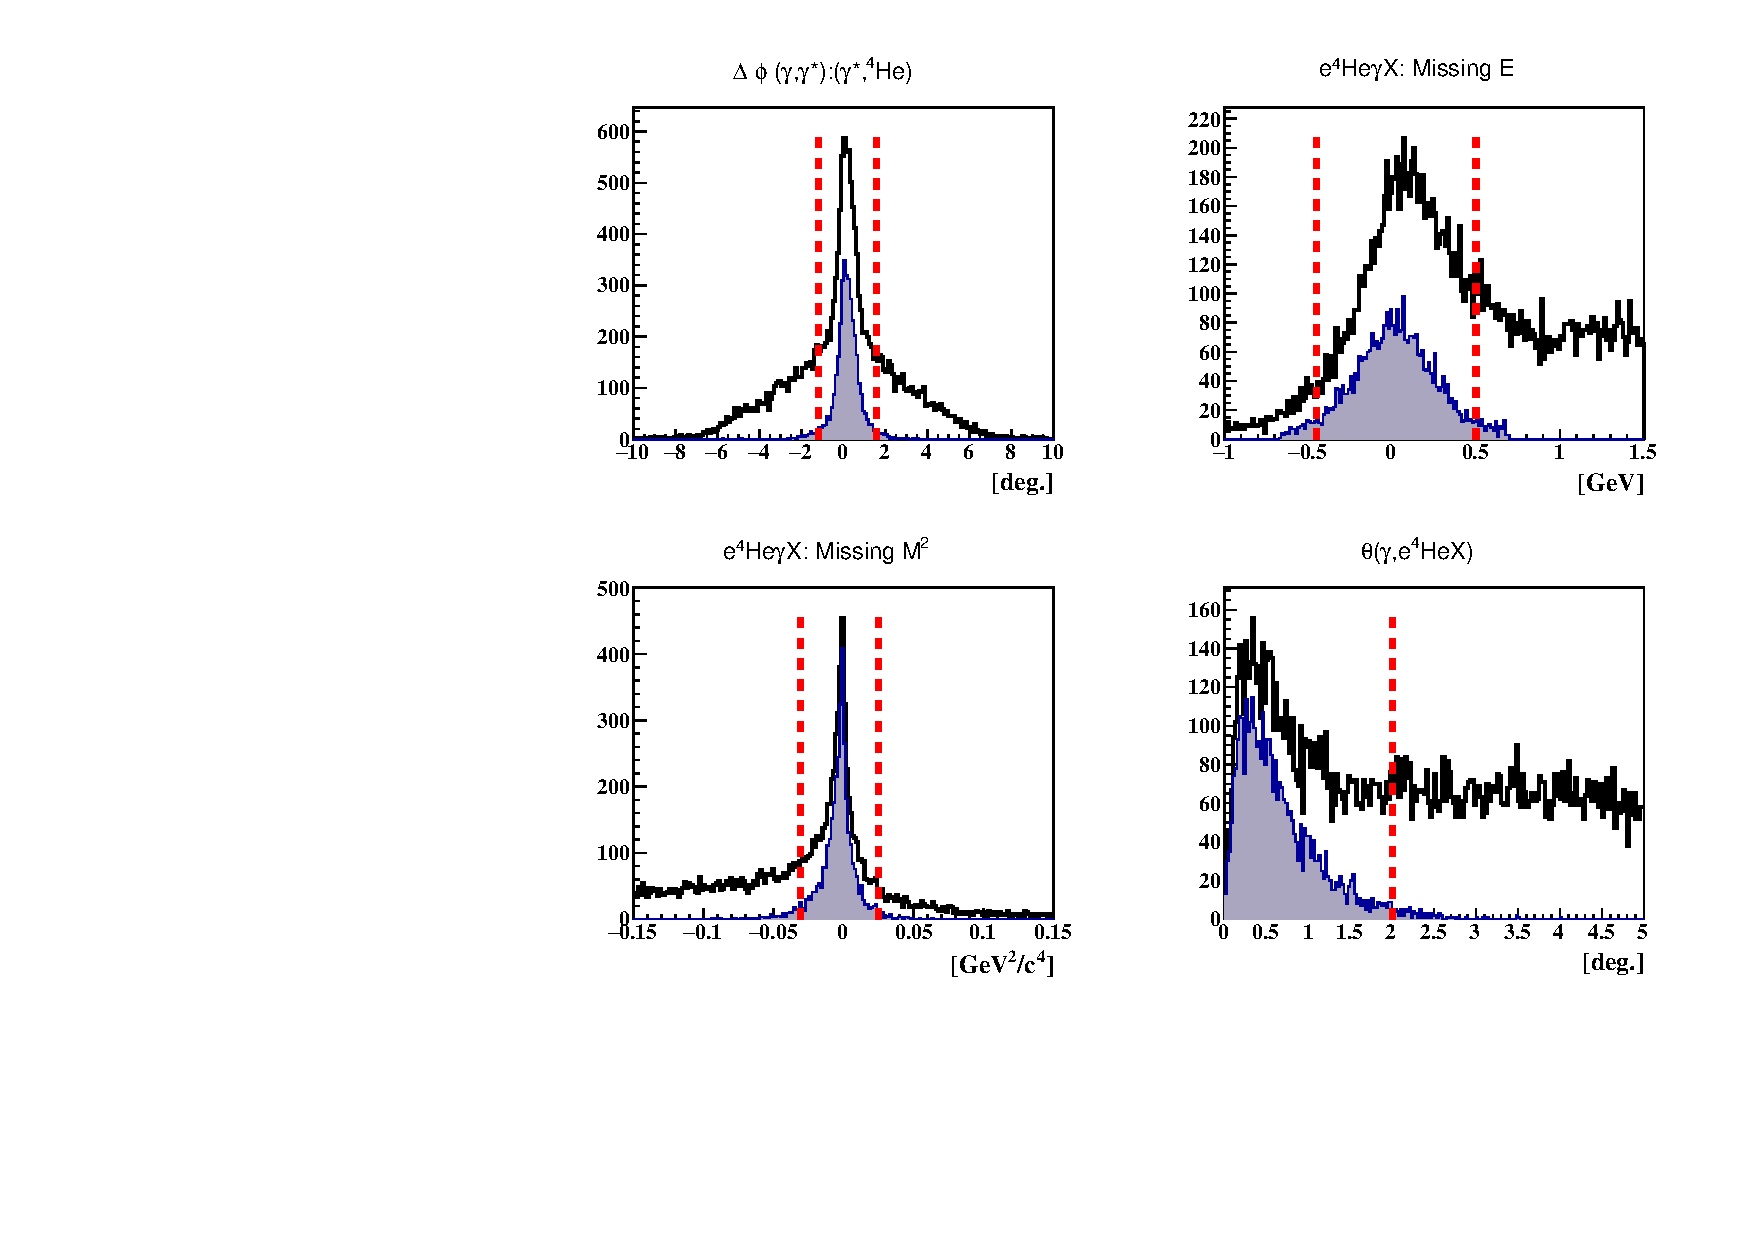
\includegraphics[width=8.9cm]{figs/coh_exc_cuts.pdf}
\caption{Four of the seven coherent DVCS exclusivity cuts. The black 
distributions represent the coherent DVCS events candidate. The shaded 
distributions represent the events which passed all the exclusivity cuts except 
the quantity plotted. The vertical red lines represent the applied exclusivity 
cuts. The distributions from left to right and from top to bottoms are: $\Delta 
\phi$, missing energy and missing mass squared in $e'^4He'\gamma X$, and the 
cone angle ($\theta$) between the measured and the calculated photons.}
\label{fig:kin-cuts}
\end{figure}
After all the requirements on the individual final state particles of the 
coherent DVCS events and the exclusivity cuts, we ended up with about 3500 
events. Figure \ref{fig:kin-coverage} presents the ($Q^{2}$,$x_{B}$) and 
($Q^{2}$,$-t$) kinematic coverage of the collected DVCS events. 

\begin{figure}[tb]
\hspace{-0.45cm}
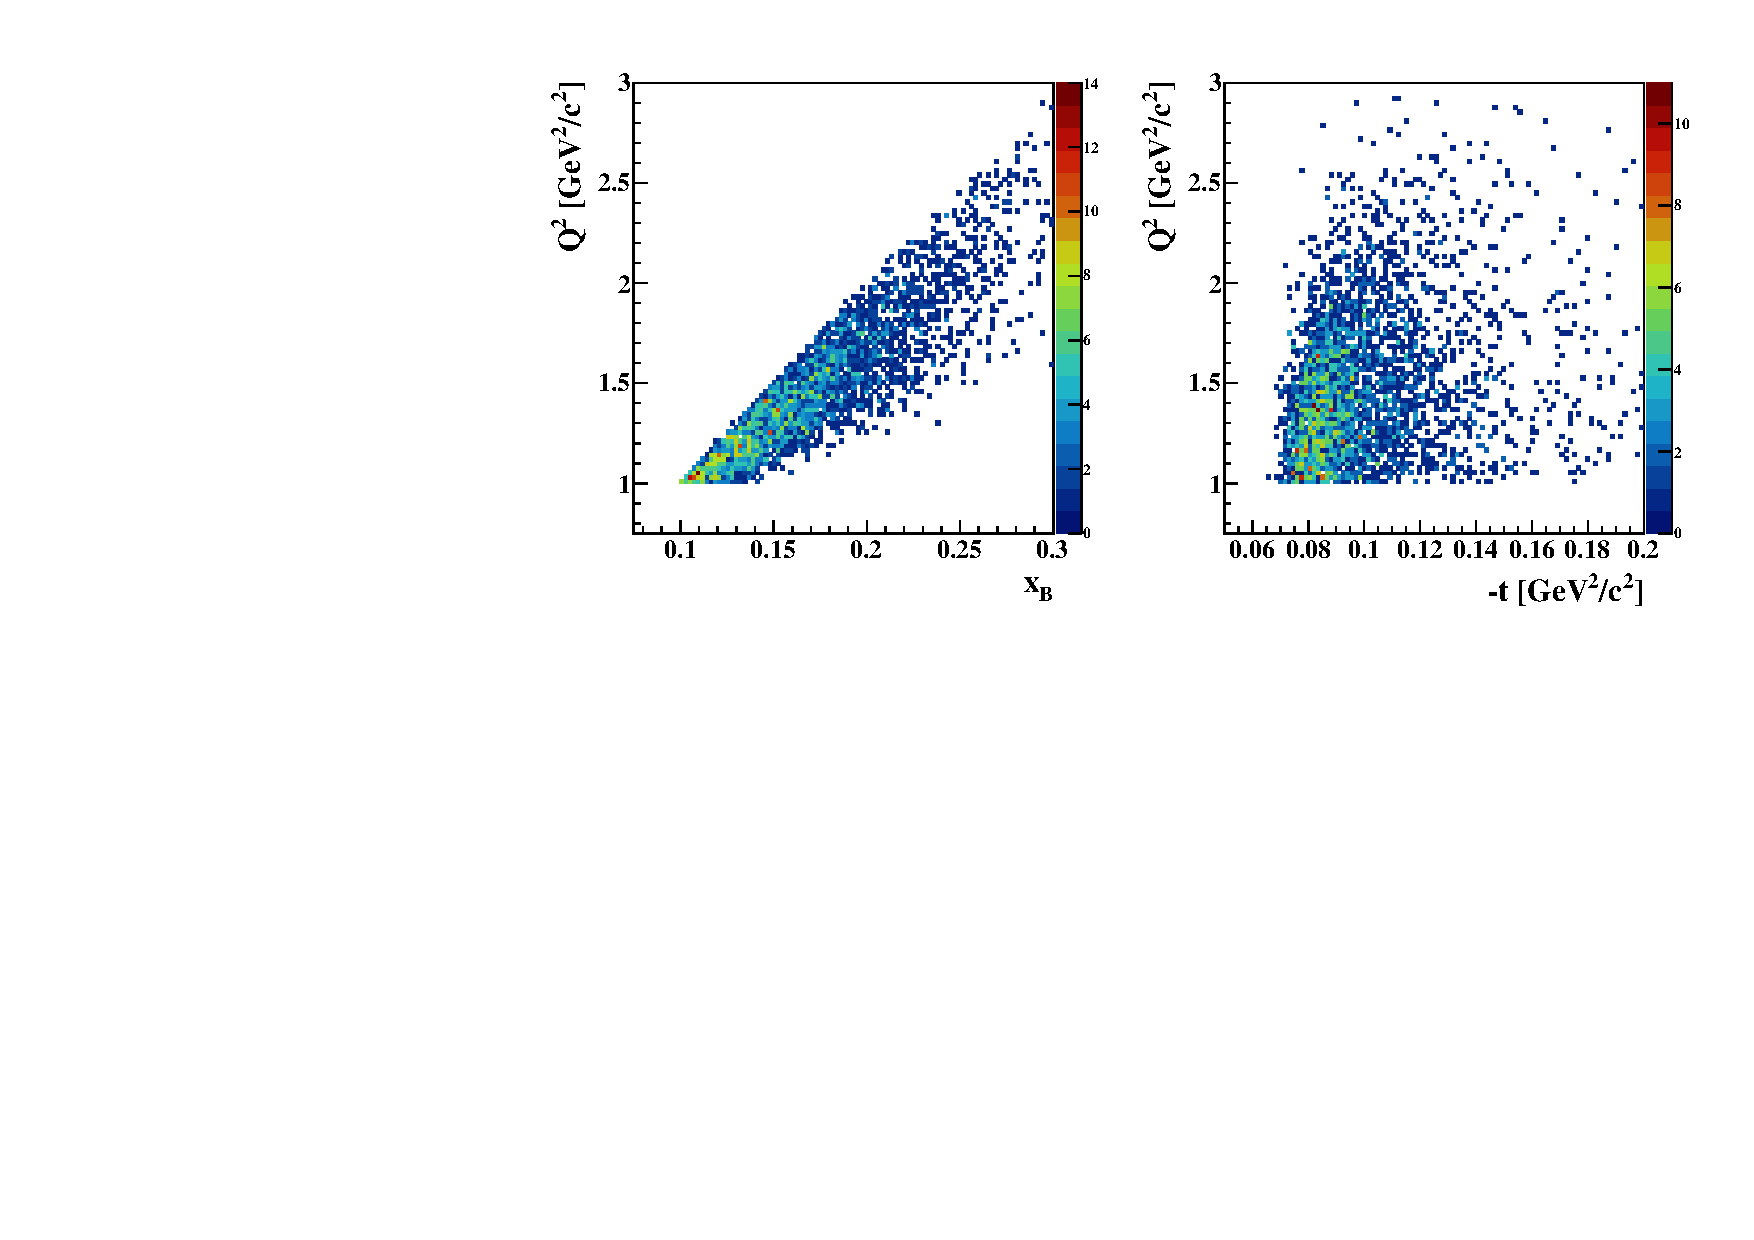
\includegraphics[width=9.0cm]{figs/Q2_xB_t_Coh.pdf}
\caption{The $Q^{2}$ as a function of $x_{B}$ (left) and the $Q^{2}$ as a 
function of $-t$ (right) for the identified coherent DVCS events after the 
exclusivity cuts.}
\label{fig:kin-coverage}
\end{figure}

%asymmetries
Even with all the previously presented exclusive cuts, the selected events are
not all true DVCS events. We identified several background contributions to the 
coherent DVCS process, in particular accidental events and exclusive Deeply 
Virtual $\pi^0$ Production (DV$\pi^0$P). The accidental events where the 
different particles come from different events are suppressed by the limited 
phase space allowed by the exclusivity cuts. We estimate the accidental events 
to represent 4.1\% of our sample. This relatively large number is due to the 
small cross section of the DVCS. We evaluated this contribution by selecting 
events passing all our cuts but with particles originating from different 
vertices. Regarding the DV$\pi^0$P, which can easily be mistaken with DVCS when 
one of the two photons of the $\pi^0$ decay is produced at low energy in the 
laboratory frame. To estimate the importance of this background, we developed 
an event generator that we calibrated to match our measured experimental yield 
of exclusive $\pi^0$. We used this generator together with a GEANT3 simulation 
of our detection system to estimate the ratio of acceptance between DV$\pi^0$P 
where the two photons are detected and those where only one photon is detected 
and would pass our DVCS selection cuts. This ratio obtained from simulation is 
then multiplied by the measured yield of DV$\pi^0$P events, indicating a 
contamination of 2 to 4\%. The study of systematics errors showed that the main 
contributions come from the choice of the DVCS exclusivity cuts (8\%) and the 
large binning size (5.1\%). However added quadratically, these errors sum up to 
10\%, which remain for all bins well below the statistical errors.

$A_{LU}$ can be simplified in terms of the collected number of events in each 
beam-helicity state ($N^{+}$, $N^{-}$) as:
\begin{equation}
A_{LU} = \frac{1}{P_{B}} \frac{N^{+} - N^{-}}{N^{+} + N^{-} }.
\end{equation}
where $P_{B}$ is the beam polarization, and $N^{+}$ and $N^{-}$ are the number 
of DVCS events detected with positive and negative electron helicity with 
respect to the beam direction. The statistical uncertainty of $A_{LU}$ is
\begin{equation}
   \sigma_{A_{LU}} = \frac{1}{P_{B}} \sqrt{ \frac{1 - (P_{B}A_{LU})^{2}}{N}}
\end{equation}
where $N (N^{+} + N^{-}) $ is the total number of measured events.

Due to our limited statistics only, a two-dimensional binning is carried out in 
this work. The strongest dependence of $A_{LU}$ is on the azimuthal angle 
($\phi$). Thus, the coherent measured ranges of $Q^{2}$, $x_{B}$ and $t$ are 
binned statistically into three bins. Then, the identified DVCS events in each 
bin are binned into nine bins in $\phi$. Therefore, we are left
with $Q^{2}$-$\phi$ bins integrated over the full ranges of $x_{B}$ and $t$, 
$x_{B}$-$\phi$ bins integrated over $Q^{2}$ and $t$, and $t$-$\phi$ bins 
integrated over $Q^{2}$ and $x_{B}$.

Figure \ref{fig:alu} presents the coherent $A_{LU}$ for the three
sets of two-dimensional bins. The asymmetries are fitted with the form of
equation \ref{eq:A_LU-coh}, where the real and the imaginary part of the CFF
$\mathcal{H}_{A}$ are the free parameters in the fit. Figure \ref{fig:alu90} 
shows the $Q^2$, $x_{B}$, and $-t$-dependencies of the fitted $A_{LU}$ signals 
at $\phi$~=~90$^{\circ}$. The $x_{B}$ and $-t$-dependencies are compared to 
theoretical calculations performed by S.~Liuti and K.~Taneja 
\cite{simonetta_2}. Their model relies on the impulse approximation and uses 
advanced spectral function of the nuclei to calculate the nuclear GPDs and then 
the observables. The calculations were carried out at slightly different 
kinematics than ours but provide already some guidance. The experimental 
results appear to have larger asymmetries compared to the calculations.  These 
differences may arise from nuclear effects which are not taken into account in 
the model, such as long-range interactions. Our measurements also agree with 
those of HERMES, considering their large uncertainties.


\begin{figure}[tb]
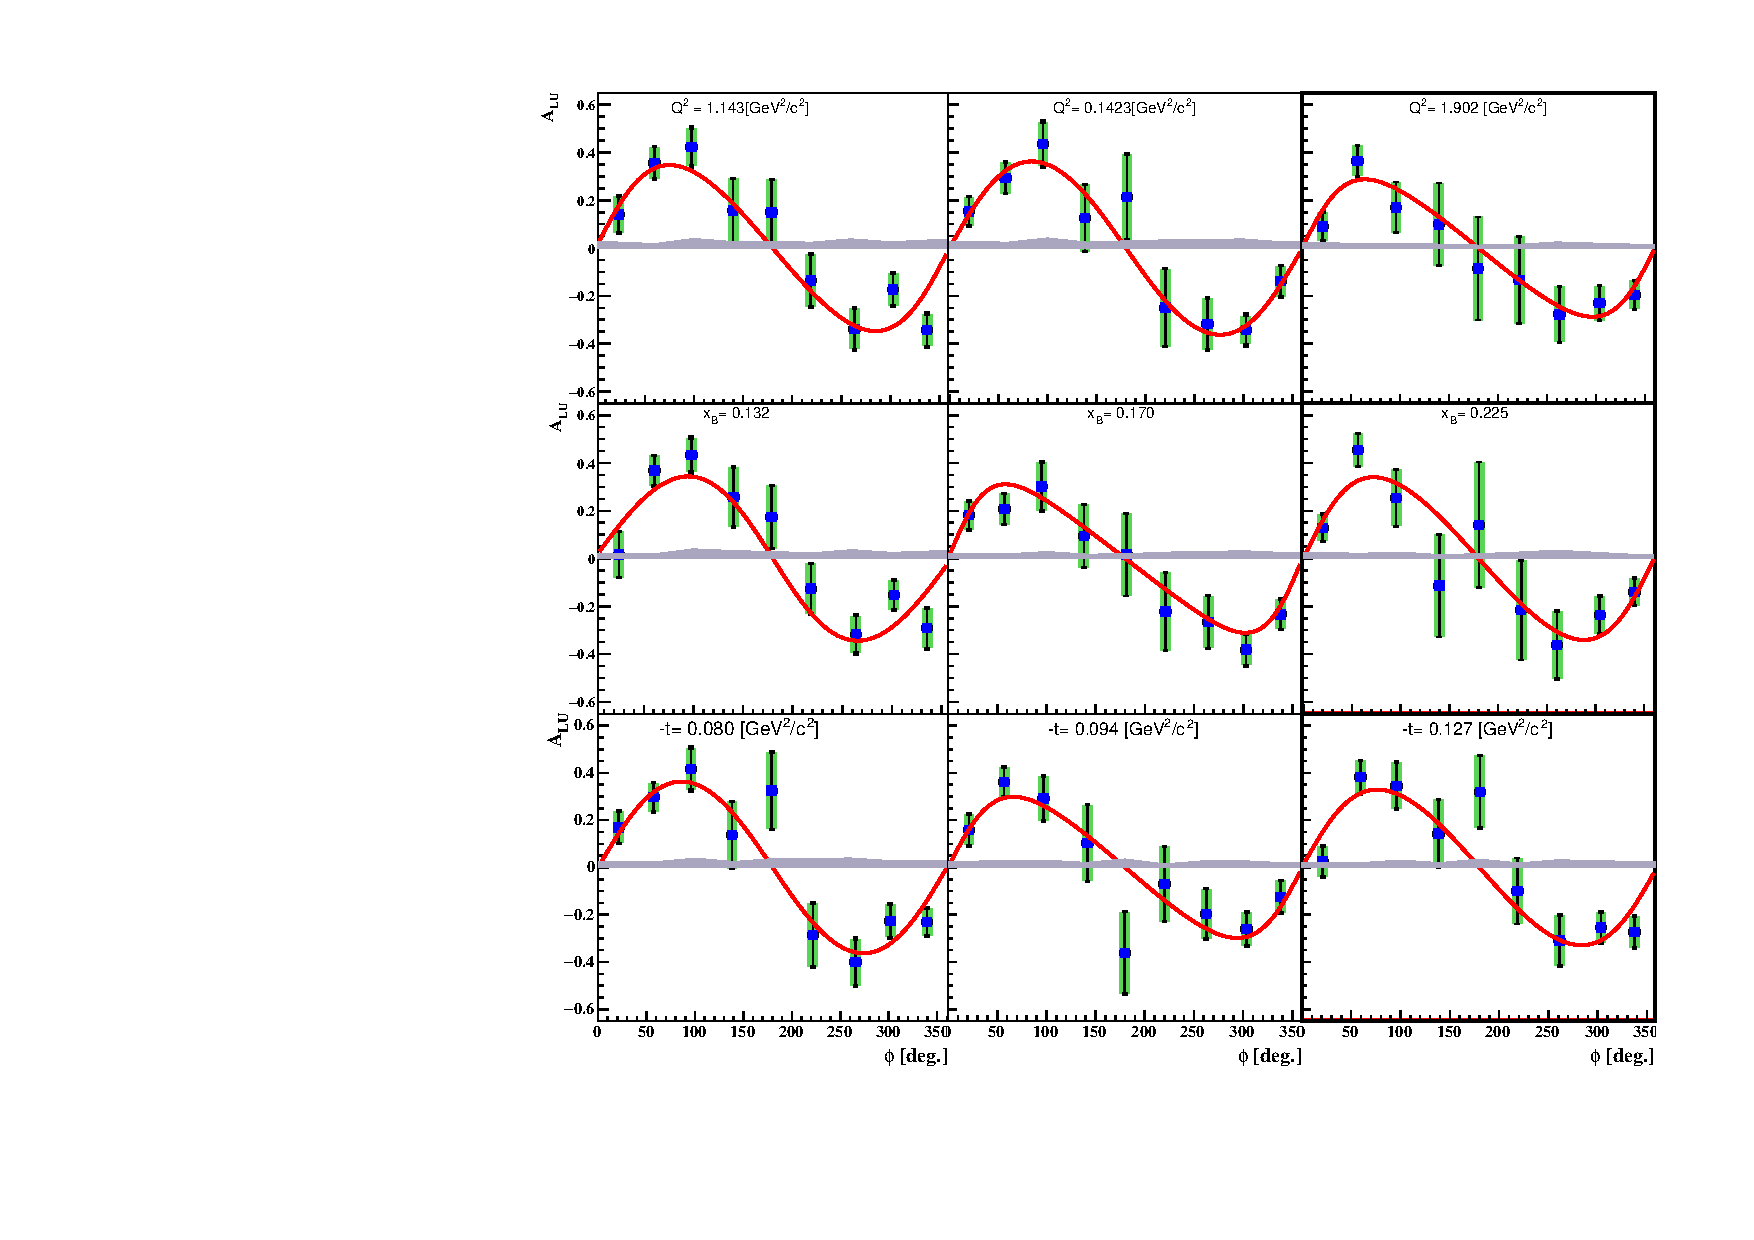
\includegraphics[width=8.9cm]{figs/coherent-ALU.pdf}
\caption{The coherent $A_{LU}$ as a function of $\phi$ in
   $Q^{2}$(top panel), $x_{B}$ (middle panel), and $-t$ (bottom panel) bins.  
   The error bars represent the statistical and the systematic uncertainties 
   added quadratically, shown on top in green are error bars representing only 
   the statistical uncertainties. The bluish-gray bands represent the 
   systematic uncertainties, including the normalisation systematic 
uncertainties. The red curves represent fits in the form of equation 
\ref{eq:A_LU-coh}.}
\label{fig:alu}
\end{figure}

\begin{figure}[tb]
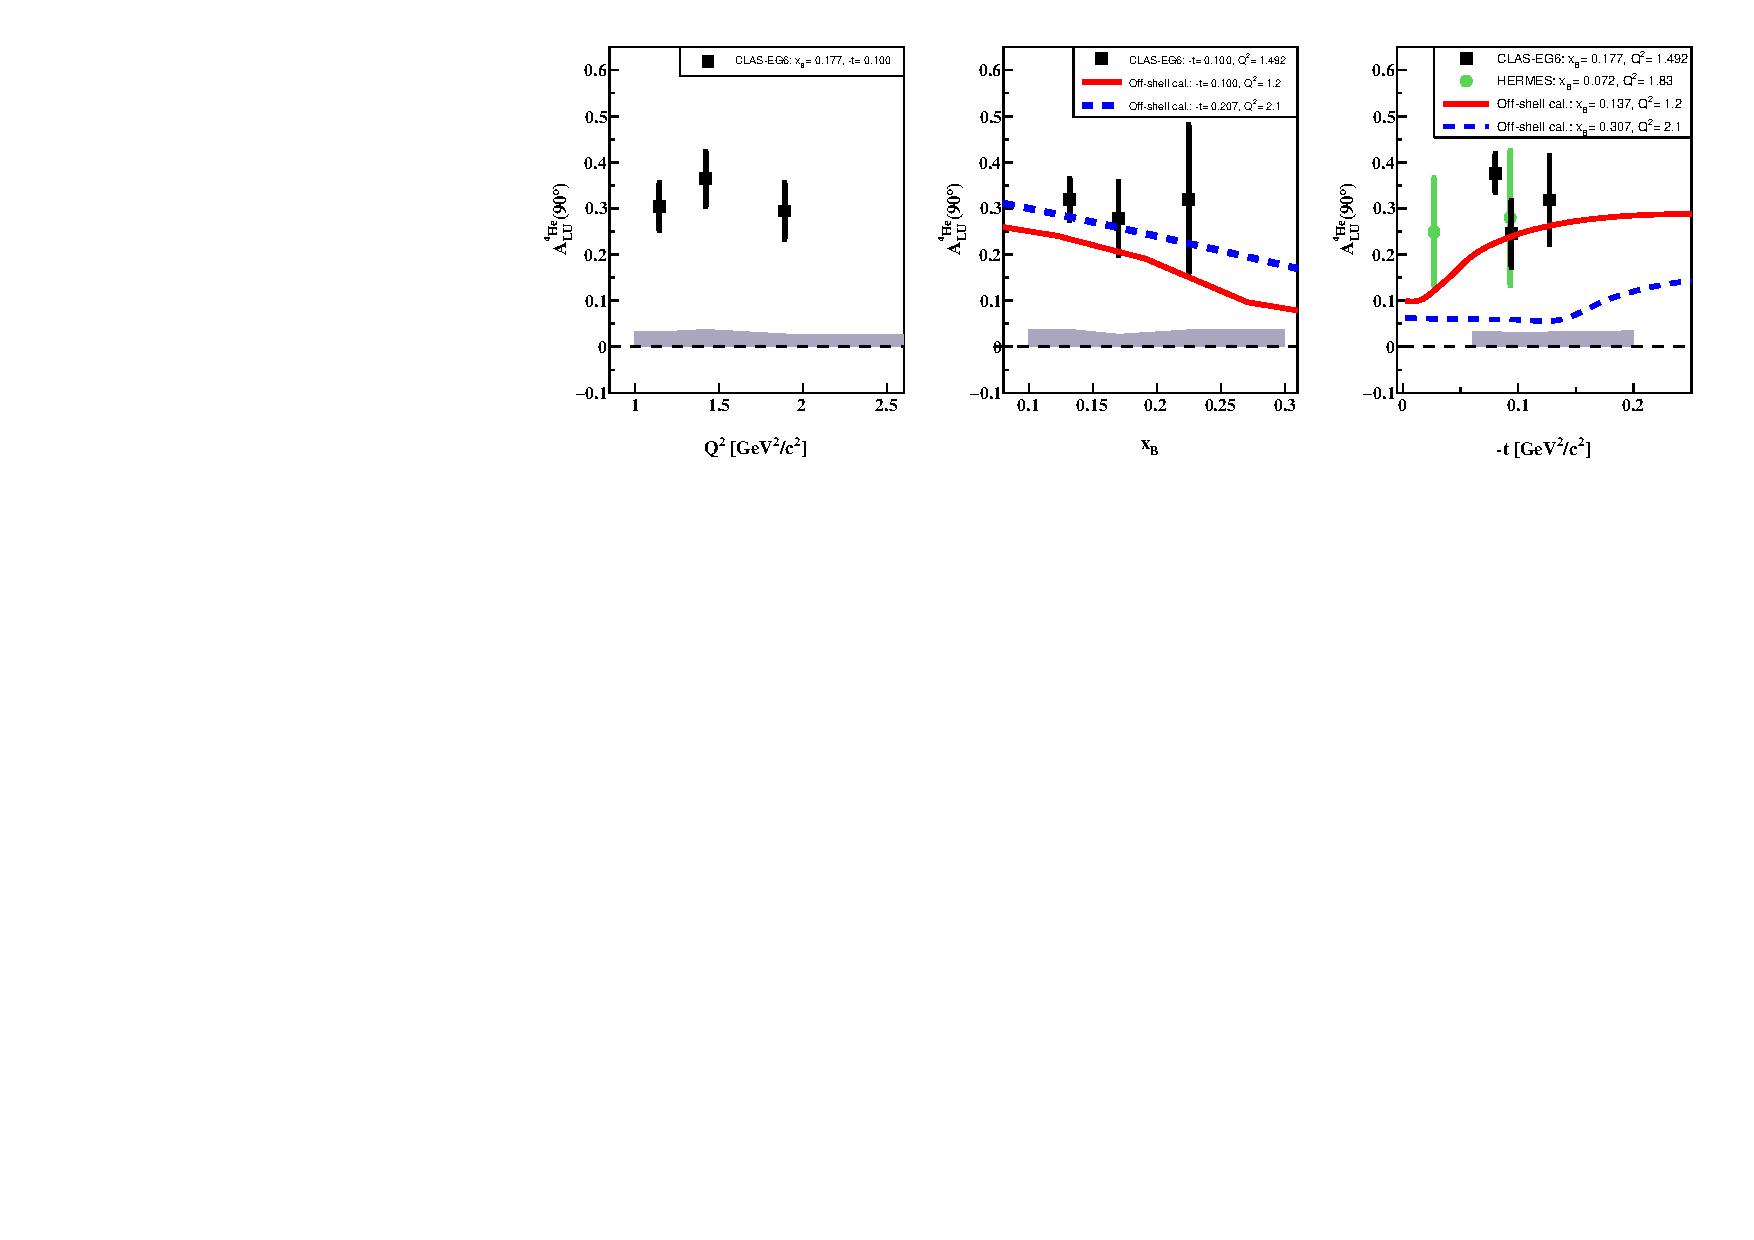
\includegraphics[width=8.9cm]{figs/coherent-ALU_90.pdf}
\caption{The $Q^{2}$ (left), $x_{B}$ (middle), and $-t$-dependencies (right) of
   the coherent $A_{LU}$ at $\phi$~=~90$^{\circ}$ (black squares). On the 
   middle plot: the full-red and the dashed-blue curves are theoretical 
   calculations from \cite{simonetta_2}. On the right: the green circles are 
   the HERMES $-A_{LU}$ (positron beam was used) inclusive measurements 
   \cite{HERMES_BSA}, the colored curves represent theoretical calculations 
from \cite{simonetta_2}.}
\label{fig:alu90}
\end{figure}

As has been advertised previously, the $^4$He CFF $\mathcal{H}_A$ can be 
extracted from fitting the experimentally measured coherent $A_{LU}$ in a 
totally model independent way, which is not the case of nucleon targets. For 
the later, four CFFs exist and extracting them is always made by making 
limitations according some theoretical models and by neglecting some CFFs 
\cite{Jo:2015ema}. Figure \ref{fig:CFF_HA} presents our extracted imaginary and 
real parts of the CFF $\mathcal{H}_A$ as function of the kinematical variable 
($Q^{2}$, $x_B$,$-t$), and compared to some theoretical calculations.

\begin{figure}[tb]
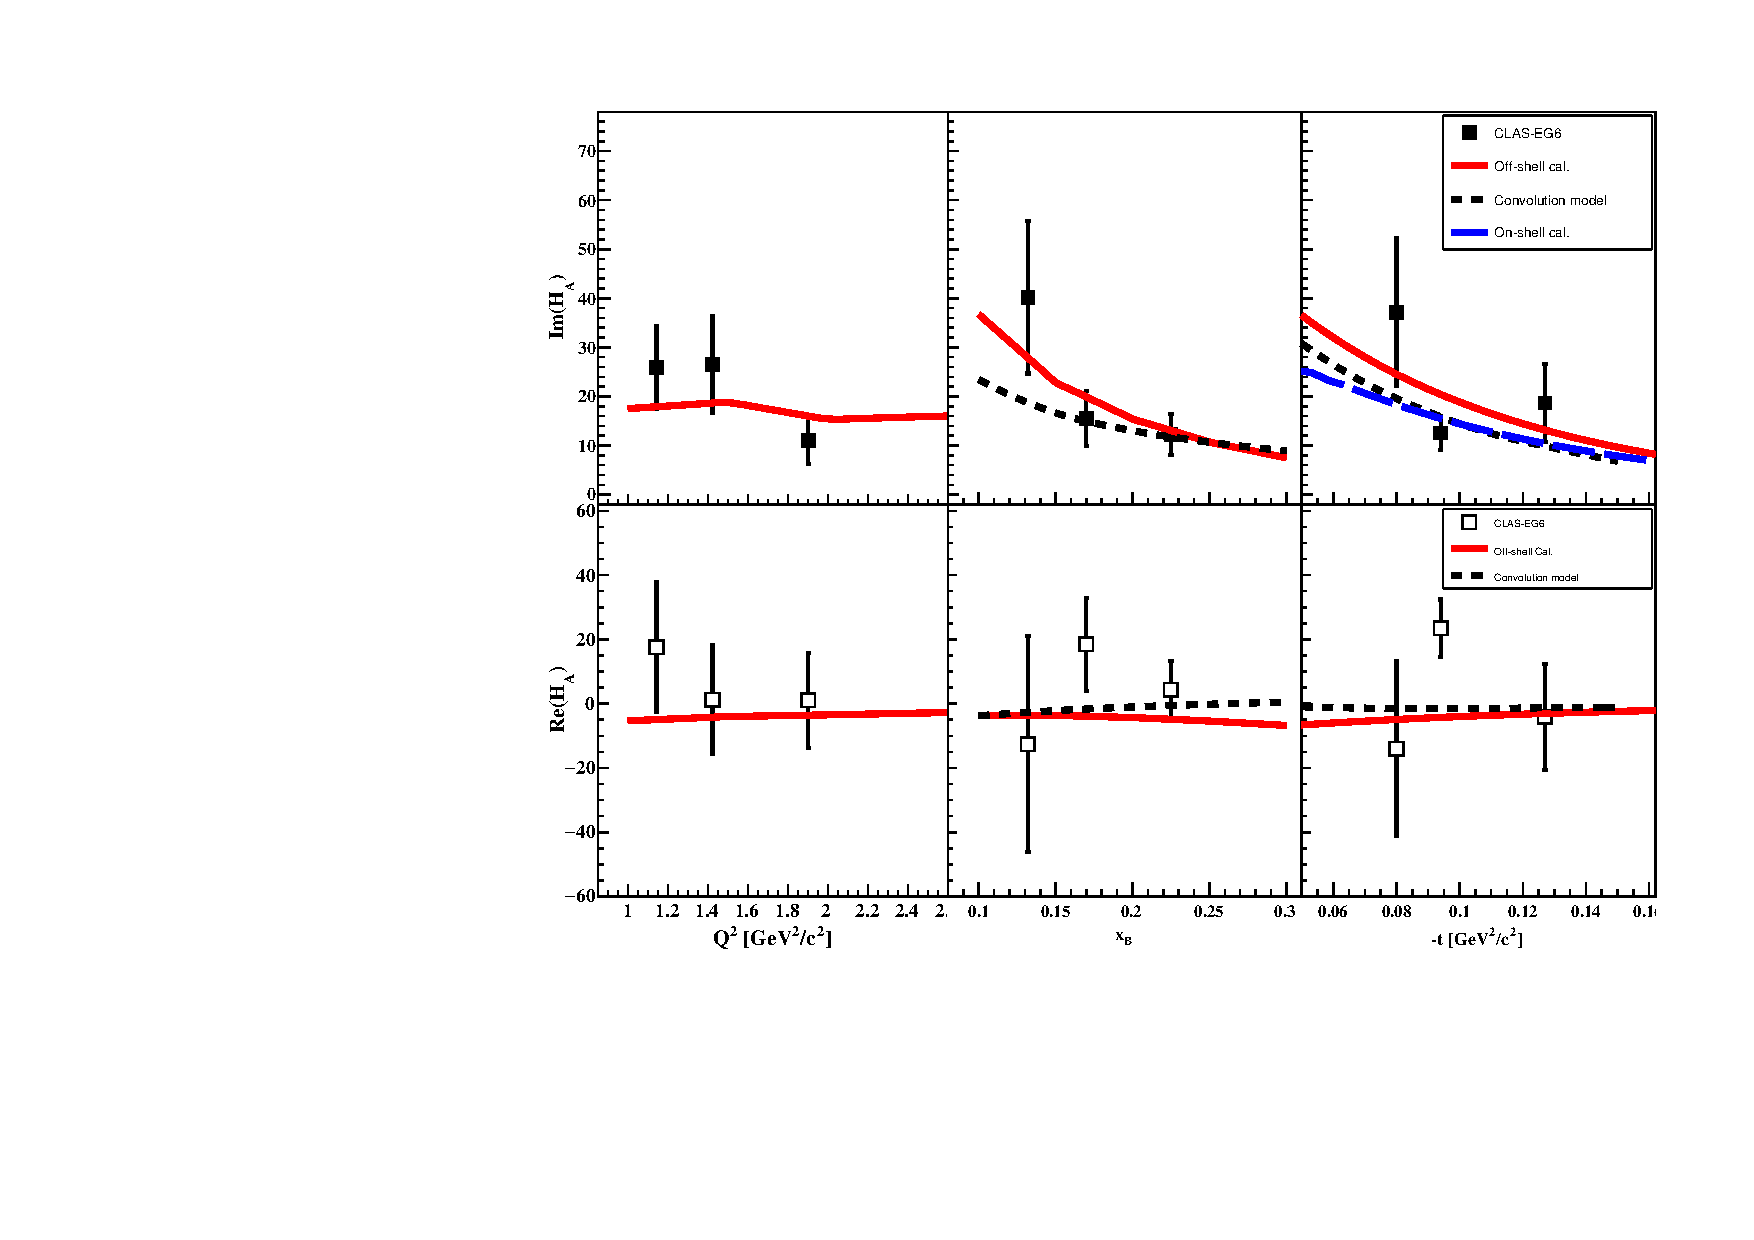
\includegraphics[width=8.9cm]{figs/Coherent_CFF.pdf}
\caption{The model-independent extraction of the imaginary (top panel) and
real (bottom panel) parts of the $^4$He CFF $\mathcal{H}_A$, as functions of
$Q^{2}$ (right panel), $x_B$ (middle panel), and $t$ (left panel). The full red 
curves are calculations based on an on-shell model from
\cite{Vadim_priv}. The black-dashed curves are calculations from a convolution 
model based on the VGG model for the nucleons' GPDs \cite{Guidal_priv}. The 
blue long-dashed curve on the top-right plot is from
an off-shell model based on \cite{GonzalezHernandez:2012jv}.}
\label{fig:CFF_HA}
\end{figure}

We display in figure \ref{fig:CFF_HA} calculations for $\mathcal{H}_A$ from 
three GPD models: On-shell, Convolution, and off-shell models. In the On-shell 
model \cite{Vadim_priv}, a nucleus is assumed to be composed of 
non-relativistic non-interacting nucleons, and these nucleons interact 
independently with the probe. For the nucleons, the GPDs are modeled according 
to the dual parametrization \cite{Guzey:2006xi}. In the Convolution model, the 
same assumption has been made for the nucleus, while the nucleon GPDs were 
extracted from the VGG model, which is based on the double distributions ansatz 
\cite{DD_model}. The Off-shell model \cite{GonzalezHernandez:2012jv} relies on 
the impulse approximation also, but uses advanced spectral function of the 
nuclei that accounts for all configurations of the final nuclear system and the 
binding effects between the nucleons.

In figure \ref{fig:CFF_HA}, within the given uncertainties, the extracted CFF 
shows a slight dependence on $Q^{2}$, $x_B$, and $-t$, which are in agreement 
with the theoretical calculations. One can see a difference between the 
precision of the extracted imaginary and real parts, which is expected because 
$\alpha_2$ is suppressed compared to $\alpha_0$ contribution. However, we note 
that the error bars are finite and that the fit converge without placing any 
bound on the CFF, which is necessary on proton targets.


%conclusion
In summary, we presented the first exclusive measurement of the coherent DVCS 
off $^4$He using CLAS spectrometer, supplemented with an inner calorimeter, a 5 
Tesla solenoid, and a specially designed radial TPC. This dataset represents a 
unique source for the nuclear DVCS global dataset, which will be used to 
constrain GPD models. The measured beam-spin asymmetries show a very strong 
signal and allowed to perform the first fully model-independent extraction of 
the $^4$He CFF $\mathcal{H}_A$. The extracted CFFs, while limited by 
statistics, are in a good agreement with the available GPD models. This opens 
many new perspectives to study the nuclear structure within the GPDs framework 
and pave the way for future more precise measurements at JLab 12~GeV program 
and possibly at the Electron-Ion Collider (EIC) to achieve better understanding 
of the nuclear effects.

%Acknowledgments

We acknowledge the staff of the Accelerator and Physics Divisions at Jefferson 
Lab for making this experiment possible. This work is supported by the U.S.  
Department of Energy, Office of Science, Office of Nuclear Physics contract 
DE-AC05-06OR23177.

\begin{thebibliography}{99}

\bibitem{Burkardt:2000za} 
  M.~Burkardt,
  Phys.\ Rev.\ D {\bf 62}, 071503 (2000)
  Erratum: [Phys.\ Rev.\ D {\bf 66}, 119903 (2002)]

\bibitem{Diehl:2002he} 
  M.~Diehl,
  Eur.\ Phys.\ J.\ C {\bf 25}, 223 (2002)
  Erratum: [Eur.\ Phys.\ J.\ C {\bf 31}, 277 (2003)]
 
\bibitem{Belitsky:2002ep} 
  A.~V.~Belitsky and D.~Mueller,
  Nucl.\ Phys.\ A {\bf 711}, 118 (2002)

\bibitem{Burkardt:2005hp} 
  M.~Burkardt,
  Phys.\ Rev.\ D {\bf 72}, 094020 (2005)

\bibitem{Stepanyan:2001sm}
S.~Stepanyan {\it et al.} [CLAS Collaboration],
Phys.\ Rev.\ Lett. {\bf 87}, 182002 (2001).

\bibitem{Airapetian}
A. Airapetian {\it et al.} [HERMES Collaboration],
Phys.\ Rev.\ Lett. {\bf 87}, 182001 (2001);
JHEP {\bf 1207}, 032 (2012);
JHEP {\bf 1006}, 019 (2010);
JHEP {\bf 0806}, 066 (2008);
Phys.\ Lett.\ B {\bf 704}, 15 (2011);
Phys.\ Rev.\  D {\bf 75}, 011103 (2007);
JHEP {\bf 0911}, 083 (2009);
Phys.\ Rev.\ C {\bf 81}, 035202 (2010);
JHEP {\bf 1210}, 042 (2012).

\bibitem{Chekanov:2003ya}
S. Chekanov {\it et al.} [ZEUS Collaboration],
Phys.\ Lett.\  B {\bf 573}, 46 (2003).

\bibitem{Aktas:2005ty}
A. Aktas {\it et al.} [H1 Collaboration],
Eur.\ Phys.\ J.\ C {\bf 44}, 1 (2005).

\bibitem{Chen:2006na} 
S.~Chen {\it et al.} [CLAS Collaboration],
Phys.\ Rev.\ Lett.\ {\bf 97}, 072002 (2006).

\bibitem{Munoz Camacho:2006hx} 
C. Mu\~noz Camacho {\it et al.} [Jefferson Lab Hall A Collaboration],
Phys.\ Rev.\ Lett. {\bf 97}, 262002 (2006).

\bibitem{Girod:2007aa} 
F.X. Girod {\it et al.} [CLAS Collaboration],
Phys.\ Rev.\ Lett. {\bf 100}, 162002 (2008).

\bibitem{Gavalian:2009} 
G. Gavalian {\it et al.} [CLAS Collaboration],
Phys.\ Rev.\ C {\bf 80}, 035206 (2009).

\bibitem{Seder:2015} 
E. Seder {\it et al.} [CLAS Collaboration],
Phys.\ Rev.\ Lett. {\bf 114}, 032001 (2015).

\bibitem{Pisano:2015} 
S.~Pisano {\it et al.} [CLAS Collaboration],
Phys.\ Rev.\ D {\bf 91}, 052014 (2015).

\bibitem{Jo:2015ema} H.~S.~Jo {\it et al.} [CLAS Collaboration],
  Phys.\ Rev.\ Lett.\  {\bf 115}, no. 21, 212003 (2015)

\bibitem{Mazouz:2007aa} 
  M.~Mazouz {\it et al.} [Jefferson Lab Hall A Collaboration],
   Phys.\ Rev.\ Lett.\  {\bf 99}, 242501 (2007)

\bibitem{Freund_Collins}
A.~Freund and J.C.~Collins, 
Phys.\ Rev.\ D {\bf 59}, 074009 (1998)

\bibitem{Ji_Osborne}
X.-D.~Ji and J.~Osborne, 
Phys.\ Rev.\ D {\bf 58}, 094018 (1998)

\bibitem{Belitsky}
A.~V.~Belitsky and A.~V.~Radyushkin, 
Phys.\ Rept.\ vol. 418 (2005)

\bibitem{Guidal:2013rya}
M.~Guidal, H.~Moutarde and M.~Vanderhaeghen,
Rept.\ Prog.\ Phys.\  {\bf 76}, 066202 (2013)

\bibitem{JSeely}
J. Seely {\it et al.} 
Phys.\ Rev.\ Lett.\ {\bf 103}, 202301 (2009)

\bibitem{CLAS_ref}
B.A. Mecking {\it et al.}, 
Nucl.\ Inst.\ and Meth.\ A 503, 513 (2003)

\bibitem{Belitsky:2001ns}
A.~V.~Belitsky, D.~Mueller and A.~Kirchner,
Nucl.\ Phys.\ B {\bf 629}, 323 (2002)

\bibitem{Kirchner:2003wt}
A.~Kirchner and D.~Mueller, 
Eur.\ Phys.\ J.\ C {\bf 32}, 347 (2003)

\bibitem{Belitsky:2008bz}
A.~V.~Belitsky and D.~Mueller,
Phys.\ Rev.\ D {\bf 79}, 014017 (2009)


\bibitem{Ellinghaus:2002zw}
F.~Ellinghaus {\it et al.} [HERMES Collaboration],
AIP Conf.\ Proc.\  {\bf 675}, 303 (2003)

\bibitem{eg6_note}
M. Hattawy {\it et al.} (CLAS-EG6 Working Group), 
CLAS internal analysis note, 2016.

\bibitem{simonetta_2}
S.~Liuti and K.~Taneja, 
Phys.\ Rev.\ C {\bf 72}, 032201 (2005)

\bibitem{HERMES_BSA}
A. Airapetian et al. (HERMES Collaboration), 
Phys.\ Rev.\ C {\bf 81}, 035202 (2010)

\bibitem{Vadim_priv}
Private communications with V.~Guzey based on: 
V.~Guzey, Phys.\ Rev.\ C {\bf 78}, 025211 (2008).

\bibitem{Guzey:2006xi}
V.~Guzey and T.~Teckentrup,
Phys.\ Rev.\ D {\bf 74}, 054027 (2006)

\bibitem{Guidal_priv}
Private communications with M.~Guidal based on: 
M.~Guidal, M.~V.~Polyakov, A.~V.~Radyushkin and M.~Vanderhaeghen, 
Phys.\ Rev.\ D {\bf 72}, 054013 (2005).

\bibitem{DD_model}
I.~V.~Musatov and A.~V.~Radyushkin, 
Phys.\ Rev.\ D {\bf 61}, 074027 (2000).

\bibitem{GonzalezHernandez:2012jv}
Private communications with S.~Liuti based on: 
J.~O.~Gonzalez-Hernandez, S.~Liuti, G.~R.~Goldstein and K.~Kathuria,
Phys.\ Rev.\ C {\bf 88}, no. 6, 065206, (2013).


\end{thebibliography}

\end{document}
